\documentclass[a4paper,11pt]{article}
\usepackage{latexsym}
\usepackage{hyperref}
\usepackage{graphicx}
\usepackage{float}
\usepackage[MeX]{polski}
\usepackage[utf8]{inputenc}
\usepackage{geometry}
\usepackage{hyperref}
\usepackage{subcaption}
\usepackage{natbib}
\usepackage[nottoc,numbib]{tocbibind}
 \geometry{
 a4paper,
 left=20mm,
 top=30mm,
 }
\author{Adam Gonstal, Kamil Kolasa, Rafał Kornel, Konrad Maliszewski, Anna Olechowska}
\title{Poszukiwanie mikrosoczewek grawitacyjnych}
\frenchspacing
\newcommand{\ak}{\hspace{0.7 cm}}
\renewcommand{\abstractname}{Abstrakt}
\bibliographystyle{plainnat}
\setcitestyle{authoryear,open={(},close={)}}
\begin{document}
\maketitle
\newpage
\begin{abstract}
\nocite{*}
\ak Poniżej opisany projekt studencki polegał na analizie fragmentu danych z projektu OGLE III w celu znalezienia zjawisk mikrosoczewkowania grawitacyjnego.  Autorom zostały udostępnione dane z teleskopu w Las Campanas w Chile, dotyczące m.in. pomiarów jasności dla ok. $260$ tysięcy  gwiazd, zbieranych na przestrzeni ok. $6$ lat. W ramach projektu utworzony został algorytm analizujący dane dla każdej gwiazdy i zwracający wykresy zależności jasności od czasu dla tych gwiazd (krzywe blasku), które według algorytmu mogły dawać efekt soczewki. Około $27$\% (24 na 88) zwróconych krzywych blasku zostało przez autorów pracy zakwalifikowanych jako potencjalne rzeczywiste przypadki mikrosoczewkowania grawitacyjnego.
\end{abstract}
\tableofcontents
\newpage
\section{Wstęp}
\subsection{Wstęp teoretyczny}
\ak Zjawisko soczewkowania grawitacyjnego wynika z zakrzywienia czasoprzestrzeni przez masy się w niej znajdujące. Konsekwencją tego jest poruszanie się promieni świetlnych po zakrzywionych torach, tj. najkrótszych możliwych, w przestrzeni Mińkowskiego. W związku z tym, w sytuacji gdy w okolicach linii łączącej źródło światła (np. galaktykę) z obserwatorem znajdzie się odpowiednio duża masa, światło biegnie omijając taką masę, co przedstawia Rysunek \ref{Fig1}. 

\begin{figure}[H]
\centering
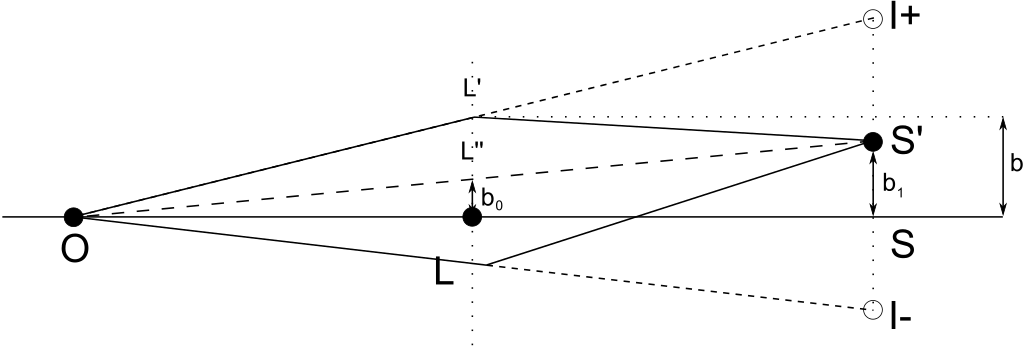
\includegraphics[width=0.9\textwidth]{Lens.jpeg}
\caption{Przykład zjawiska soczewkowania, gdzie źródło S' jest obserwowane jako dwa obrazy I+ i I- \citet{Lens}.}
\label{Fig1}
\end{figure}

\ak Obraz źródła widziany przez obserwatora może ulec różnym deformacjom, tj. rozciągnięciu, przemieszczeniu, kilkukrotnemu odbiciu, a także wzmocnieniu, co w przypadku tego projektu jest najistotniejszym aspektem soczewkowania. Przykłady takiego zjawiska przedstawiają Rysunki \ref{Fig2} i \ref{Fig3}.
\begin{figure}[H]
\begin{subfigure}{0.5\textwidth}
\centering
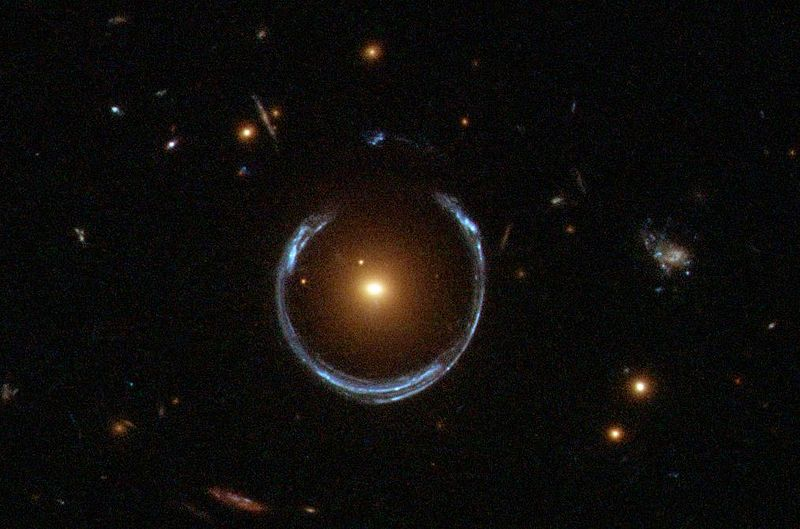
\includegraphics[width=0.9\linewidth,height=5cm]{Horseshoe.jpeg}
\caption{Galaktyka LRG 3-757 soczewkująca obraz galaktyki znajdującej się za nią \citet{Horseshoe}}
\label{Fig2}
\end{subfigure}
\hspace{0.5cm}
\begin{subfigure}{0.5\textwidth}
\centering
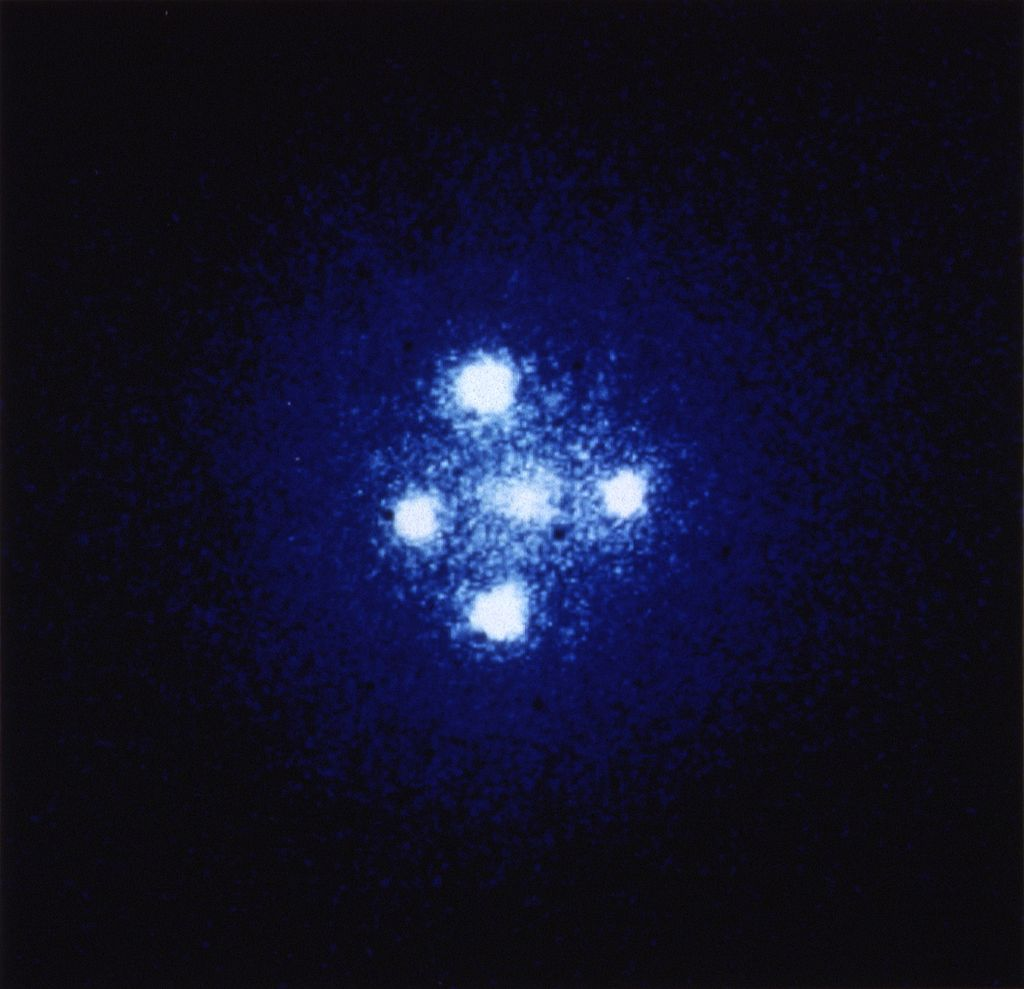
\includegraphics[width=0.9\linewidth,height=5cm]{Cross.jpeg}
\caption{Kwazar Q2237+030 soczewkowany przez galaktykę ZW 2237+030, tzw. krzyż Einsteina \citet{Cross}}
\label{Fig3}
\end{subfigure}
\caption{Przykłady deformacji obrazu spowodowane soczewkowaniem grawitacyjnym}
\end{figure}
\ak W szczególnych przypadkach, gdy masa soczewkująca jest stosunkowo nieduża, a jej tor ruchu przecina bądź jest bardzo bliski torowi promieni świetlnych od źródła do obserwatora, efekty deformacji obrazu mają zbyt małe rozmiary kątowe, by udało się je zaobserwować z Ziemi. W takich sytuacjach jedyną obserwowalną konsekwencją zajścia soczewki jest wzmocnienie jasności. Ten specyficzny rodzaj soczewkowania nazywany jest mikrosoczewkowaniem grawitacyjnym. Przykładem jego może być obiekt z pobliskiej galaktyki wysyłający ku Ziemi promieniowanie elektromagnetyczne, na którego drodze znajduje się masywna planeta. Wzmocnienie można wyrazić jako wielkość $\mu$, będącą ilorazem strumienia światła bez wzmocnienia oraz z wzmocnieniem. Ponieważ natężenie światła $I$ jest stałe w czasie, będzie to wyłącznie iloraz kątów bryłowych, z których światło dociera do  obserwatora.\\
\begin{equation}
\centering
\mu=\frac{Id\Omega}{Id\Omega_{0}}=\frac{d\Omega}{d\Omega_{0}}
\label{Eq_1}
\end{equation}
\flushleft
\ak Wzmocnienie można również dobrze opisać za pomocą odległości $u$ źródła światła od soczewki, którą można przedstawić za pomocą kilku parametrów, które dla danej soczewki można przyjąć jako stałe w trakcie trwania zjawiska. Wspomniane parametry geometryczne mają wpływ na $t_{E}$, tj. czas Einsteina. Wielkość $b$ jest wielkością analogiczną do parametru zderzenia i także jest stała. Czas $t_{0}$ jest momentem największego wzmocnienia, z kolei jedyną zmienną we wzorze \ref{Eq_2} jest czas {t}.
\begin{equation}
\centering
u(t)=\sqrt{\left(\frac{t-t_{0}}{t_{E}}\right)^{2}+b^{2}}
\label{Eq_2}
\end{equation}
\ak Znając już zależność $u(t)$ można powiązać ją ze wspomnianym wcześniej wzmocnieniem $\mu$, tj. wyprowadzić wzór \ref{Eq_3}, zwany także krzywą Paczyńskiego. Przykładową krzywą Paczyńskiego przedstawia Rysunek \ref{Fig_4}.
W skali sześciu lat mikrosoczewka trwająca ok. $70$ dni widocznie wyróżnia się skokiem jasności w trakcie trwania zjawiska, co było punktem wyjściowym przy konstrukcji algorytmu i zostanie opisane dokładniej w kolejnych rozdziałach.
\begin{equation}
\centering
\mu(u)=\frac{u^{2}+2}{u\sqrt{u^{2}+4}}
\label{Eq_3}
\end{equation}
\flushleft
\subsection{Projekt OGLE}

\ak Projekt OGLE  tj. ,,Optical Gravitational Lensing Experiment'' jest projektem naukowym prowadzonym w obserwatorium Las Campanas w Chile, przez Obserwatorium Astronomiczne Uniwersytetu Warszawskiego, w ramach którego m.in. wykonywane są pomiary jasności gwiazd, mające na celu poszukiwanie zjawisk mikrosoczewkowania. 

\ak Projekt kierowany jest przez prof. Andrzeja Udalskiego, a jego zasadniczym obszarem obserwacji są rejony w pobliżu centrum naszej galaktyki. Od początku istnienia projektu (kwiecień 1992 roku) zaobserwowano: 20 nowych planet pozasłonecznych, ponad 4000 zjawisk mikrosoczewkowania oraz kilkaset tysięcy nowych gwiazd zmiennych\footnote{Dane ze strony internetowej projektu: \textit{http://www.astrouw.edu.pl/index.php/ogle-artykul}}. Projekt jest aktualnie (od marca 2010 roku) w czwartej fazie realizacji. Poprzednie fazy miały miejsce w latach: 1992-1995 (OGLE-I), 1997-2001 (OGLE-II), 2001-2009 (OGLE-III) i wiązały się ze stosowaniem innych detektorów.
 

\section{Analiza danych}
\subsection{Dane}
\ak Dane na których oparty jest nasz projekt studencki pochodzą z projektu OGLE-III i zawierają 280.000 plików tesktowych, w których znajduje się około 2400 pomiarów jasności zebranych na przestrzeni 6-ciu lat. Każdy pomiar był reprezentowany przez linijkę tekstu, zawierał datę pomiaru, jasność gwiazdy oraz błąd pomiarowy. Warto wspomnieć, że jakość pomiarów jest daleka do ideału i musieliśmy przefiltrować dane, najpierw odrzucając błędy grube. Wśród nich były pomiary o jasności 99 mag, co nie jest fizyczne i było spowodowane najprawdopodobniej sposobem obróbki zdjęć zebranych przez sensor ccd.
\subsection{Struktura programu}
\ak Do analizy danych napisaliśmy program w języku Python. Dokładny kod znajduje się na platformie github \url{https://github.com/wolf3213/Projekt-Astrolensing}. Składa się on z kilku części:
\begin{enumerate}
\item ,,Main'', czyli cześć główna programu, w której podawane były nazwy katalogów, służył do uruchamiania programu.
\item ,,Predictor'', czyli plik zawierający klasę odpowiedzialną za działanie algorytmu.
\item ,,Parser'', czyli plik zawierający klasę służącą do parsowania plików wejściowy do obiektów na których potem operował algorytm.
\item ,,Curve'', czyli plik zawierający klasę odpowiedzialną za przechowywanie danych, tworzenie wykresów i wstępne odrzucanie szumów.
\end{enumerate} 
W programie wykorzystaliśmy następujące biblioteki:
\begin{enumerate}
	\item Numpy - do przechowywania pomiarów,
	\item Matplotlib - modułu pyplot do rysowania pomiarów oraz dopasowanych krzywych,
	\item Scipy - funkcji curve_fit z modułu optimize, do dopasowania parametrów krzywej Paczyńskiego.
\subsection{Odsiew szumu}
\ak Właściwa część programu zaczynała się dopiero po wczytaniu danych. Wstępnie odfiltrowywał on wszystkie potencjalnie nienadające się do obróbki dane. Obejmowało to dane, które:
\begin{enumerate}
\item Zawierały pomiary jasności o wartości większej/równej 99 magnitudo 
\item Zostały wykonane między 1. a 2137., oraz  2450. i 2500. dniem (właściwie indeksem daty) trwania projektu OGLE. Musieliśmy je usunąć, ponieważ zawierały zbyt dużą ilość błędnych pomiarów, za bardzo odstających od średniej jasności. Usunięcie kilkudziesięciu pomiarów nie wpłynęło negatywnie na analizę danych, oraz nie zmniejszyło informacji zawartych w pomiarach. 
\end{enumerate}

\subsection{Format danych - klasa 'Curve'}
\ak Wczytane i przefiltrowane dane były przez nas przechowywane jako obiekty klasy 'Curve'. Zawierała ona pola, takie jak:
\begin{enumerate}
	\item times - listę z biblioteki numpy (np.array) zawierającą daty pomiarów, uporządkowaną rosnąco,
	\item mags - listę z bilbioteki numpy zawierającą wartości jasności gwiazdy,
	\item errors - listę z biblioteki nupmy zawierającą błędy pomiarowe,
\end{enumerate}
		oraz kilka innych, mniej znaczących pól (np mag_mean - średnia jasność gwiazdy, mag_std - odchylenie standardowe jasności).
Obiekty posiadały również kilka przydatnych funkcji, ułatwiających obróbkę danych (i nie tylko), m.in:
\begin{enumerate}
	\item update_data - metoda służąca do przypisania obiektowi nowych danych (np. pozbawionych szumu) oraz obliczenia jeszcze raz wartości średnich, odchyleń standardowych itp.
	\item cut_points - metoda usuwająca pomiary z zadanych przedziałów czasowych,
	\item plot - metoda odpowiedzialna za rysowanie wykresów krzywych,
	\item fit - metoda obliczająca parametry najlepszego dopasowania krzywej Paczyńskiego.


\subsection{Opis algorytmu}
\ak Program, operując już na nieodrzuconych danych, oblicza dla pomiarów jasności danej gwiazdy: odchylenie standardowe  $\sigma_{mag}$ i średnią $m_0$. Następnie  sprawdza, które pomiary jasności $m$ spełniają nierówność

\begin{equation}
m<\sigma_{mag}\cdot A+m_0 
\label{Eq_4}
\end{equation}
to znaczy są jaśniejsze niż średnia plus pewna wielokrotność $\sigma_{mag}$ i zlicza je, przy czym $A$ jest arbitralnie ustaloną dodatnią liczbą. Następnie dla punktów spełniających nierówność, liczy odchylenie standardowe po czasie $\sigma_t$, oraz średni czas $t$ tych punktów. \\ 
Wartość $A$ jest skorelowana z głębokością soczewek, których szukamy. Im większa wartość $A$, tym głębsze soczewki program będzie znajdował, w drugą stronę, dla małych wartości $A$ program powinien wykryć soczewki płytkie. Niestety w rzeczywistości płytkie soczewki często nie były wykrywane, ponieważ były głębokości szumu. W rezultacie udało nam się znaleźć jedynie głębsze soczewki.  \\

\ak Program determinował czy krzywa jest soczewką na podstawie wielkości $\sigma_t$. Jest to szerokość rozkładu punktów odrzuconych - spełniających nierówność 
		(\ref{Eq_4}) wokół wyliczonej średniej, która rozumiana może być jako moment największego pojaśnienia soczewki. Ustalając górną granicę szerokości rozkładu odrzuconych punktów kierowaliśmy się założeniem, że soczewki które nas interesują, tzn te głębokie, trwają zazwyczaj bardzo krótko, często nie dłużej niż kilkadziesiąt dni. Jeśli więc algorytm wykrył, że puntky pomiarowe spełniające nierówność (\ref{Eq_4}) są położone blisko średniej ich czasu, zwracał krzywą jako podejrzaną o soczewkowanie. Aby zrozumieć dlaczego algorytm działa, trzeba uzmysłowić sobie fakt, że dla krzywej bez soczewki, punkty spełniające (\ref{Eq_4}) to pomiary zaszumione, a te są statystycznie równo rozłożone po całej krzywej. Zatem dla krzywej bez soczewki wartość $\sigma_t$ powinna być duża.

\subsection{Napotkane trudności}
Algorytm przedstawiony przez nasz zespół nie był pozbawiony mankamentów. Jego głównym celem było jak najsprawniejsze przesianie danych, które z pewnością nie są soczewkami. Głównym problemem, z którym musięliśmy się skonfrontować była konieczność ręcznego przejrzenia plików, które program zakwalifikował jako potencjalne soczewki. Przykładową krzywą blasku, którą program zakwalifikował jako soczewkę, a która w rzeczywistości jest gwiazdą zmienną przedstawia rysunek poniżej.
\begin{figure}[H]
\begin{subfigure}{0.5\textwidth}
\centering
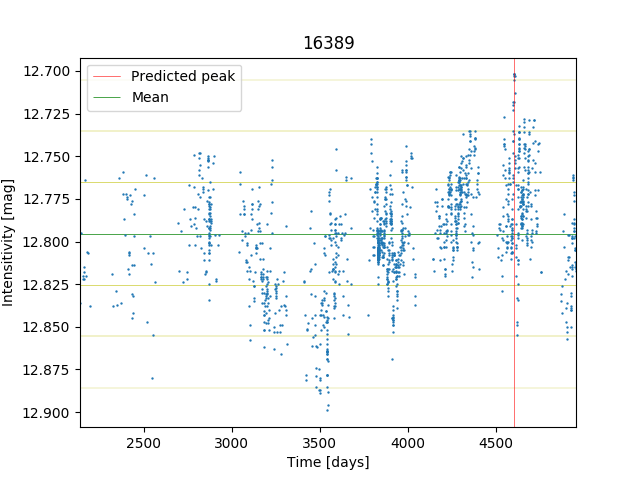
\includegraphics[width=\linewidth,height=5.5cm]{16389.png}
\label{Fig_10}
\end{subfigure}
\hspace{0.25cm}
\begin{subfigure}{0.5\textwidth}
\centering
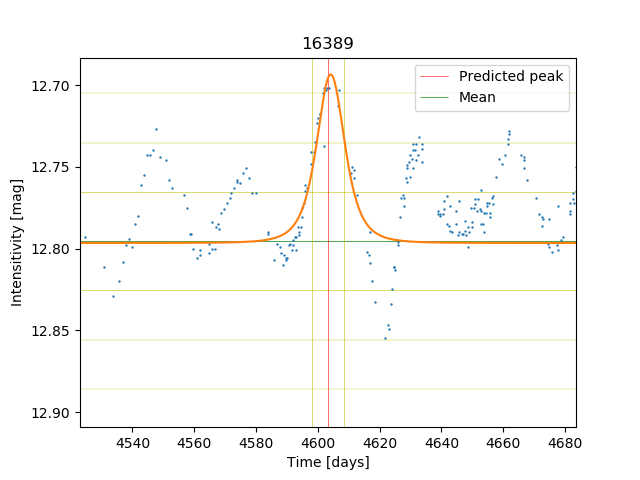
\includegraphics[width=\linewidth,height=5.5cm]{16389_v.png}
\label{Fig_11}
\end{subfigure}
\caption{Gwiazda zmienna w pliku 16389 zakwalifikowana przez algorytm jako soczewka}
\end{figure}

Wśród podejrzanych krzywych znajdowało się też dużo takich, których pomiary w określonych przedziałach czasowych były bardzo niedokładne i odbiegające od średniej. Zniwelowaliśmy ten problem wycinając część pomiarów.

\section{Rezultaty}
		\ak W celu oszacowania jaki błąd pierwszego rodzaju jest generowany przez nasz program, wzięliśmy potwierdzone soczewki udostępnione na stronie OGLE, i sprawdziliśmy ile z nich zostanie wykryte przez program. Nasz program, dla wartości $A = 3$ oraz górnej granicy $\sigma_t$ punktów spełniających (\ref{Eq_4}) wykrył 26 soczewek na 36 plików. Pliki na których przeprowadzone zostały testy zostały zapisane w folderze code/lens/ na naszym repozytorium na githubie.
\subsection{Znalezione soczewki}
\ak Uruchomiliśmy program na pełnym zbiorze dostarczonych danych przy parametrach: 
$$A=3\textrm{, } T=30$$
\ak Według nas znaleźliśmy , przy tych parametrach 24 soczewki, 31 wykresów jasności jest do dalszej dyskusji, oraz przypadkowo 14 gwiazd zmiennych. Przykładowe wykresy jasności soczewek załączone są w podsekcji ,,Wizualizacj''. 
\begin{subsection}{Wizualizacje}
	\ak Wynikiem działania programu są pliki graficzne w formacie .png, które przedstawiają dopasowaną krzywą Paczyńskiego do danych w momencie wystąpienia potencjalnej soczewki. Poziome linie koloru żółtego to kolejne wielokrotności wartości $\sigma_mag$, zaś pionowa czerwona to predykcja momentu wystąpienia największego pojaśnienia, dokonana przez algorytm. Pliki zostały przez nas przejrzane i wybrane zostały z nich te, które wizualnie najbardziej odpowiadały faktycznemu wystąpieniu soczewki. Część z nich przedstawiliśmy na rysunkach poniżej.
\begin{figure}[H]
\begin{subfigure}{0.5\textwidth}
\centering
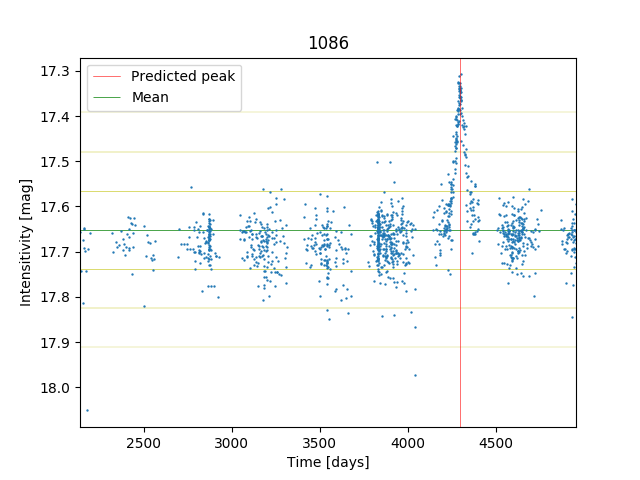
\includegraphics[width=\linewidth,height=5.5cm]{1086.png}
\label{Fig_4}
\end{subfigure}
\begin{subfigure}{0.5\textwidth}
\centering
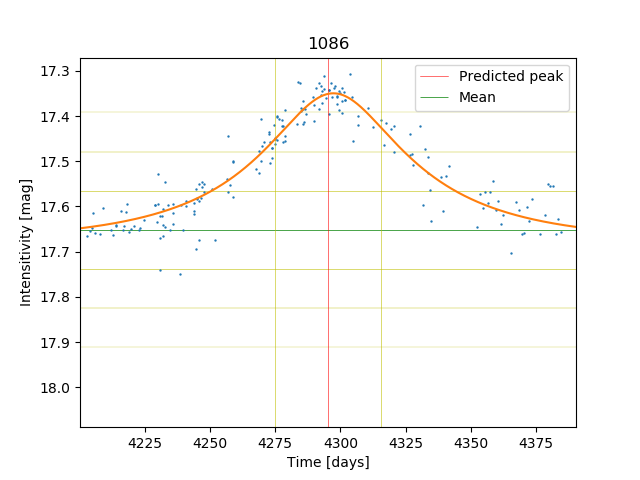
\includegraphics[width=\linewidth,height=5.25cm]{1086_v.png}
\label{Fig_5}
\end{subfigure}
\caption{Peak znaleziony wśród danych dla gwiazdy w pliku o numerze 1086 wraz z przybliżeniem i dopasowaną krzywą Paczyńskiego}
\end{figure}
\begin{figure}[H]
\begin{subfigure}{0.5\textwidth}
\centering
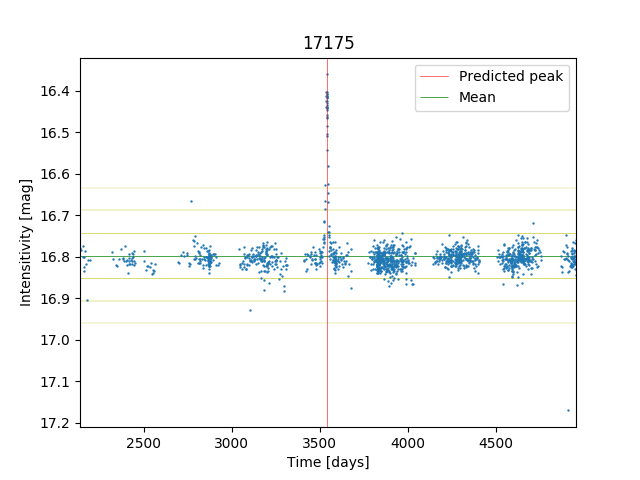
\includegraphics[width=\linewidth,height=5.25cm]{17175.png}
\label{Fig_6}
\end{subfigure}
\begin{subfigure}{0.5\textwidth}
\centering
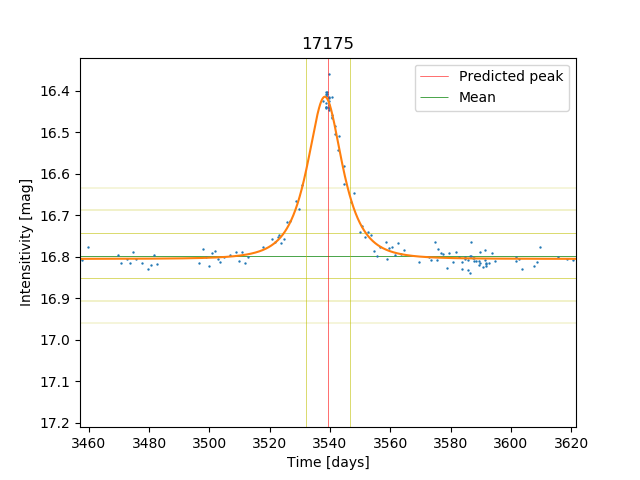
\includegraphics[width=\linewidth,height=5.25cm]{17175_v.png}
\label{Fig_7}
\end{subfigure}
\caption{Peak znaleziony wśród danych dla gwiazdy w pliku o numerze 17175 wraz z przybliżeniem i dopasowaną krzywą Paczyńskiego}
\end{figure}
\begin{figure}[H]
\begin{subfigure}{0.5\textwidth}
\centering
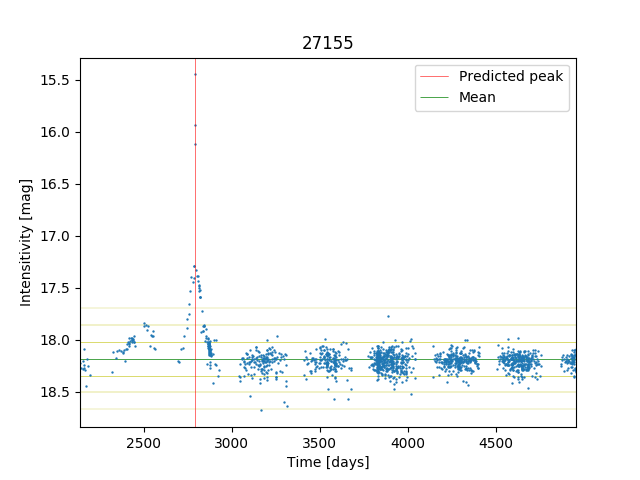
\includegraphics[width=\linewidth,height=5.25cm]{27155.png}
\label{Fig_8}
\end{subfigure}
\begin{subfigure}{0.5\textwidth}
\centering
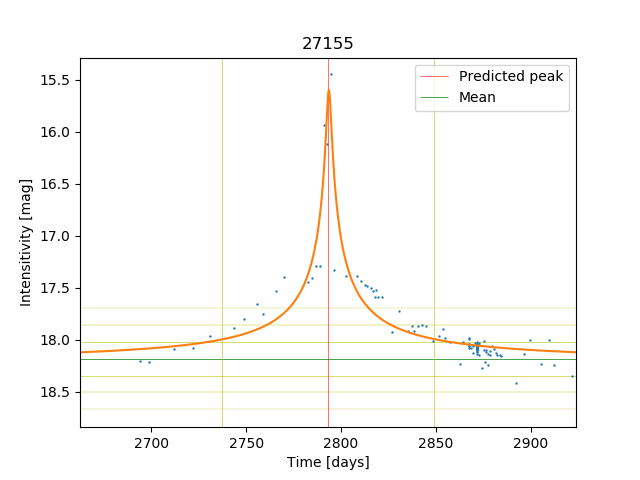
\includegraphics[width=\linewidth,height=5.25cm]{27155_v.png}
\label{Fig_9}
\end{subfigure}
\caption{Peak znaleziony wśród danych dla gwiazdy w pliku o numerze 27155 wraz z przybliżeniem i dopasowaną krzywą Paczyńskiego}
\end{figure}
\begin{figure}[H]
\begin{subfigure}{0.5\textwidth}
\centering
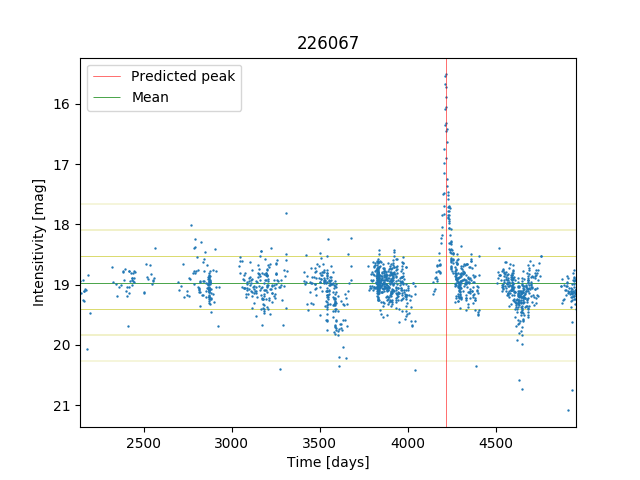
\includegraphics[width=\linewidth,height=5.25cm]{226067.png}
\label{Fig_12}
\end{subfigure}
\begin{subfigure}{0.5\textwidth}
\centering
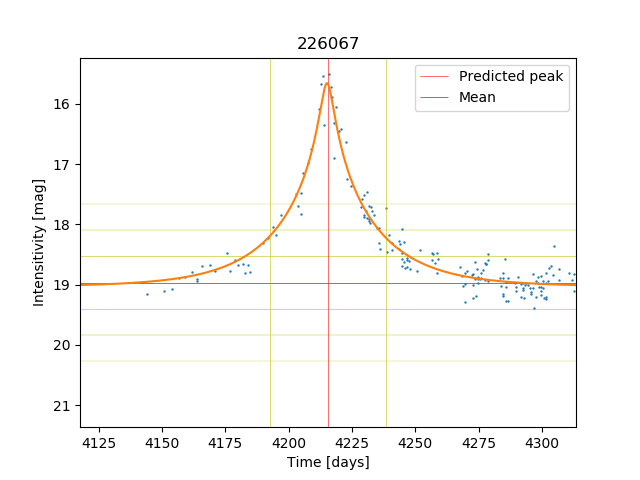
\includegraphics[width=\linewidth,height=5.25cm]{226067_v.png}
\label{Fig_13}
\end{subfigure}
\caption{Peak znaleziony wśród danych dla gwiazdy w pliku o numerze 226067 wraz z przybliżeniem i dopasowaną krzywą Paczyńskiego}
\end{figure}
\end{subsection}
\bibliography{bibliografia}
\end{document}
